
% =====================================================================
%  CHAPTER 4 — METHODOLOGY
%  Zero-Shot Nutrient and Quantity Association using
%  OCR-Guided Semantic Graph Matching
%  Moustafa Hamada | THD + USB
%
%  Build: scrbook, XeLaTeX + BibTeX. Citations: \cite{}. Cross-refs: \S\ref{}.
%
%  LABELS USED IN THIS FILE (align to your actual labels if they differ):
%    chap:methodology, sec:overview, sec:ocr, sec:classifier,
%    sec:enrichment, sec:graph, sec:association, sec:vlm-assoc
%    chap:background (Ch2), chap:evaluation (Ch5), chap:experiments (Ch6)
%    fig:pipeline-overview
% =====================================================================
% --- float placement: minimise figure whitespace (delete to revert) ---


\chapter{Methodology}\label{chap:methodology}
\DeclareRobustCommand{\mcode}[1]{\begingroup\ttfamily\detokenize{#1}\endgroup}
This chapter specifies the proposed extraction system and the design
decisions behind it. The emphasis is on \emph{what} each processing
stage produces and \emph{how} the individual components operate. The
target dataset, the annotation schema, the evaluation metrics and the
matching procedure used for scoring are deferred to
Chapter~\ref{chap:evaluation}, and all quantitative results---including
the outcome of every ablation introduced below---are reported in
Chapter~\ref{chap:experiments}. Wherever a component is presented as one
of several interchangeable variants, this chapter describes each variant
on equal footing; the comparison between them is an empirical question
answered later.

\section{System Overview and Problem Formulation}\label{sec:overview}

This section explains the task and the system as a whole. The later sections then cover each stage on its own. It is split into four parts. The first part sets out the problem, which means the input the pipeline receives and the output it has to produce. The second part gives the design principles behind the pipeline. The third part goes through the pipeline stage by stage. The fourth part presents the ablation axes and how the experiments are set up.
\subsection{Problem formulation}\label{sec:overview-problem}

The pipeline receives a single image of a nutrition or supplement label as input, denoted by \(I\). This image can be either a photograph of a label or a scan of a product package. In the first stage, the image is passed through an OCR engine, whose purpose is to convert the visible text on the label into machine-readable text tokens. Rather than treating OCR as a final extraction result, this work uses it as the starting point for a structured extraction and association pipeline. The OCR output is therefore represented as a set of detected tokens, where each token contains the recognised text together with its bounding-box coordinates in the image.

Each detected OCR token is represented as
\[
t_i = (s_i, b_i, c_i),
\]
where \(s_i\) denotes the recognised text string, \(b_i = (x_1, y_1, x_2, y_2)\) denotes the token bounding box in image coordinates, and \(c_i \in [0,1]\) is the confidence score produced by the OCR engine. The bounding box is kept because the spatial position of a token is important for later reasoning about rows, columns, neighbouring values, and contextual headers.

Although OCR engines usually return the detected tokens in some output order, this order is treated only as an initial by-product and not as a reliable layout representation. In real nutrition and supplement labels, information is frequently presented in tables, dense panels, and semi-structured regions. As a result, the interpretation of a token depends more on its spatial position than on its position in the OCR output list. This is especially important for quantities, which may be visually close to multiple nutrient names or context headers. Therefore, the pipeline does not rely on a simple reading order such as left-to-right or top-to-bottom, but instead preserves the token coordinates for later graph-based association.

After the OCR stage, the detected tokens are assigned semantic roles. This step adds meaning to the raw OCR output by identifying whether a token represents a nutrient name, a numerical quantity, a measurement unit, a contextual header, or another type of text. Formally, a classifier \(\varphi\) maps each token \(t_i\) to a role
\[
r_i = \varphi(t_i),
\]
where \(r_i\) belongs to a finite set of roles \(R\). The roles required for the final extraction are
\[
\{\textsc{nutrient},\ \textsc{quantity},\ \textsc{unit},\ \textsc{context}\} \subseteq R.
\]
In addition to these four main roles, the role set also includes auxiliary labels such as \(\textsc{nrv}\) and \(\textsc{noise}\). These auxiliary labels are useful during intermediate processing because they help the pipeline separate relevant nutritional information from surrounding text, percentages, headers, or unrelated label content.

The target output is a set of tuples \(Y(I) = \{(n, q, u, x)\}\), where \(n\) is the nutrient name, \(q\) is the numeric quantity, \(u\) is the measurement unit, and \(x\) is the context under which the quantity is stated. The context can refer, for example, to a serving, a daily dose, or a value per 100~g. The task of the system is therefore not only to detect these fields separately, but to recover the correct association between them.

The gold annotations include two additional fields that are not part of the main four-field output tuple: the nutrient reference value percentage, denoted as \texttt{nrv\_percent}, and the serving size, denoted as \texttt{serving\_size}. These fields are included in the annotation file, but they are not used in the primary output tuple defined in this chapter. The evaluation of the complete four-field tuple \((n, q, u, x)\), referred to as 4F, together with the three-field version \((n, q, u)\), referred to as 3F, is described in Chapter~\ref{chap:evaluation}.

The pipeline is tested in a zero-shot setting. In practice, this means that the system is not trained or fine-tuned on the target label images. The learning-based components are used only as pre-trained models, and the rule-based components rely on manually defined lexicons and rules. This is important for the thesis because the purpose is not to build a system that simply fits these 57 labels. The aim is to check whether the proposed OCR-guided association approach can still work on nutrition and supplement labels that were not used for training.

\subsection{Design principles}\label{sec:overview-principles}

The pipeline was designed around three practical requirements: modularity, inspectability, and the ability to operate without training on the target dataset.

The first requirement is modularity. The system is divided into separate stages, where each stage has a clear input and output. The OCR stage detects text tokens and their bounding boxes. The correction stage handles common OCR artefacts. The classifier assigns semantic roles to the tokens. The enrichment stage adds layout-based and structural information. The graph construction stage then represents the enriched tokens as nodes and their spatial and semantic relationships as edges. Finally, the association stage uses this graph to reconstruct the output tuples. This staged design makes the pipeline easier to modify and analyse. If one component needs to be improved or replaced, it can be changed without rewriting the full system. It also makes the ablation experiments more meaningful, because individual components can be exchanged while the rest of the pipeline remains unchanged.

The second requirement is interpretability. In this task, an incorrect tuple can result from different stages of the pipeline: a missed OCR token, a wrong semantic role, an incorrect graph edge, or a wrong context association. For this reason, the pipeline keeps the intermediate outputs explicit. Each token preserves its text, role, confidence score, and spatial position, while graph edges are assigned types such as row compatibility, column compatibility, adjacency, and header scope. This makes it possible to trace how a tuple was formed instead of only observing the final output.

The third requirement is zero-shot generalisation. The system should operate without training on the target label dataset. For this reason, the pipeline uses pre-trained models, rule-based components, and graph-based reasoning instead of a supervised model fitted to the 57 evaluation labels. This makes the method more suitable for labels with unseen layouts, nutrient names, or textual formats.

\subsection{Pipeline architecture}\label{sec:overview-pipeline}

Figure~\ref{fig:pipeline-overview} provides an overview of the pipeline used in this thesis. It shows the order of the main processing stages and indicates where the ablation variants are introduced.

The first stage is OCR, described in Section~\ref{sec:ocr}. It extracts text tokens from the input label image, together with their bounding boxes and confidence values. In the experiments, two OCR engines are considered: EasyOCR and PaddleOCR PP-OCRv5.

The next stage is correction and normalisation, also described in Section~\ref{sec:ocr}. This stage handles common OCR-related problems before the tokens are passed to the classifier. These problems include fused quantity--unit tokens, reference-value percentages attached to numerical values, split nutrient names, and inconsistent surface forms. The implemented corrector is \texttt{OCR corrector}. A key part of this stage is the C15 normalisation rule, which maps nutrient names to the canonical forms used later during evaluation.

After correction, the semantic role classification stage assigns a role to each token. This stage is described in Section~\ref{sec:classifier}. The roles include nutrient, quantity, unit, context, NRV, and noise. Three classifier variants are evaluated in the experiments: a rule-based classifier, a BGE-M3 embedding classifier, and a GLiNER-biomed classifier.

The enrichment stage is described in Section~\ref{sec:enrichment}. At this stage, the classified tokens are extended with additional layout and structural information. This includes the column identity, the expected role of the column, the ordinal rank of a token within its column, dosage-stream membership, and header-related flags. The stage is implemented mainly through \texttt{token enricher} and \texttt{geometry engine}.

The graph construction stage is described in Section~\ref{sec:graph}. Here, the tokens are represented as graph nodes, while the relationships between tokens are represented as typed edges. Two graph constructors are evaluated. The first, \texttt{graph constructor}, builds a simpler graph mainly from raw geometric relations. The second, \texttt{graph v2 Constructor}, uses the enriched token attributes and supports different edge-creation modes.

The final association stage is described in Section~\ref{sec:association}. Its role is to reconstruct the final nutrient tuples from the graph. The first association variant is used with the simpler graph constructor, while \texttt{graph v2 associator} is used with the enriched, geometry-aware graph. A third variant replaces graph traversal with a vision--language model association step, where the model receives an injected token table, as described in Section~\ref{sec:vlm-assoc}.

\begin{figure}[htbp]
  \centering
  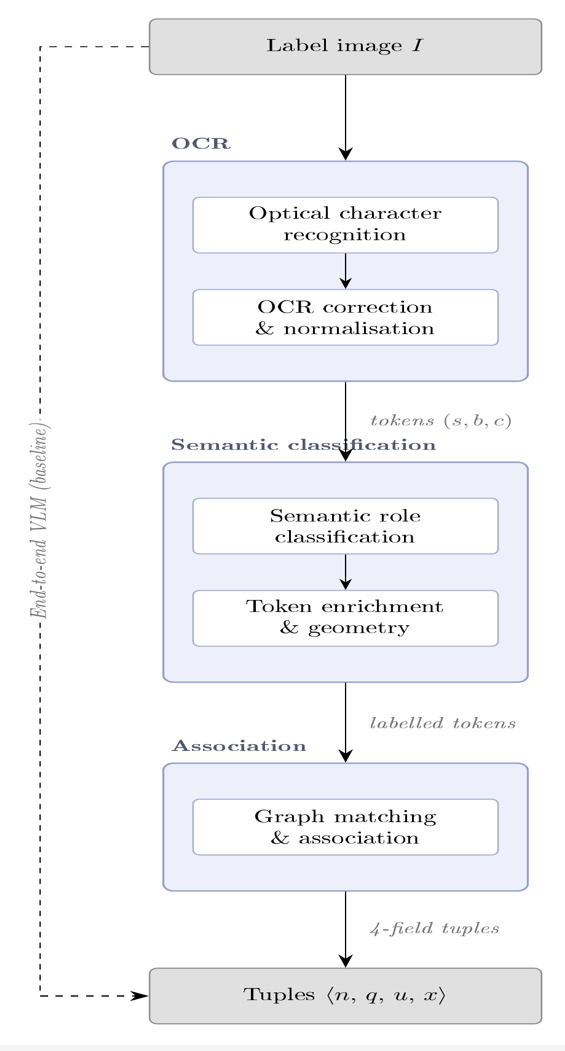
\includegraphics[width=\linewidth,height=0.80\textheight,keepaspectratio]{pipeline_overview.png}
  \caption[Pipeline overview]{%
    Overview of the proposed OCR-guided extraction pipeline. The input label image is first converted into OCR tokens, which are then corrected, classified, enriched with layout information, represented in a semantic graph, and finally associated into structured nutrient tuples. The figure also shows the main ablation points evaluated in the experiments: the OCR engine, the semantic classifier, and the association engine. The dashed branch represents the end-to-end vision--language baseline, which bypasses the modular OCR-guided pipeline.}
  \label{fig:pipeline-overview}
\end{figure}

\subsection{Ablation axes and experimental design}\label{sec:overview-ablation}

Because the pipeline is modular, the experiments are designed to test the effect of changing one stage at a time. The thesis focuses on three main ablation axes: the OCR engine, the semantic classifier, and the association engine. In addition, an end-to-end vision--language model is included as an external baseline, since it follows a different extraction strategy and does not use the modular OCR-guided pipeline.

The first ablation axis is the OCR engine. EasyOCR and PaddleOCR PP-OCRv5 are compared while keeping the remaining stages of the pipeline fixed. This comparison is performed first because OCR quality directly affects all later stages of the pipeline. The OCR engine selected from this experiment is then used in the remaining ablation experiments.

The second ablation axis is the semantic classifier. Three classifier variants are compared: the rule-based classifier, the BGE-M3 embedding classifier with cosine similarity, and the GLiNER-biomed classifier. These variants are included because they represent different design trade-offs. The rule-based classifier is fast and transparent, but depends on the coverage of the manually defined lexicon. The embedding classifier is more flexible with unseen surface forms, but can introduce semantic confusion when visually or semantically similar tokens are close together. GLiNER provides a different pre-trained zero-shot alternative, with behaviour that differs from both the rule-based and embedding-based approaches.

The third ablation axis is the association engine. The first variant uses the simpler graph constructor and traversal strategy, referred to as graph~v1. The second variant uses the geometry-aware graph constructor and traversal strategy, referred to as graph~v2. The third variant replaces graph traversal with a vision--language model association step based on an injected token table. In this VLM-association variant, the model receives the corrected token table before C15 normalisation, and C15 is applied afterwards to the model output.

After the OCR engine is fixed, the classifier and association axes are combined in a \(3 \times 3\) factorial experiment. In other words, each semantic classifier is evaluated with each association engine. The end-to-end vision--language baseline is evaluated separately, since it maps the original label image directly to output tuples and does not use the OCR-guided graph pipeline. This baseline is included to compare the proposed modular and interpretable design with a more direct black-box alternative.

One implementation detail is important for reading the experimental results. The enrichment stage is executed for all pipeline configurations, but graph~v1 does not use the enriched structural attributes. It relies only on the raw token geometry. Graph~v2, in contrast, uses the enriched token information when constructing edges. Therefore, although enrichment is present in the pipeline, not every association engine benefits from it in the same way. This distinction helps explain the performance difference between graph~v1 and graph~v2 in the experiments chapter.

The full experiment matrix, dataset description, evaluation metrics, and tuple-matching procedure are described in Chapter~\ref{chap:evaluation}. The quantitative results and ablation comparisons are reported in Chapter~\ref{chap:experiments}.

\begin{table}[htbp]
  \centering
  \caption[Implementation names and the names used in the text]{Mapping between the implementation (Python) names in the codebase and the plain-language names used in this chapter. The text uses the right-hand names; the left-hand names are listed only so each term can be traced back to the code. Model identifiers (\mcode{BAAI/bge-m3}, \mcode{Ihor/gliner-biomed-bi-large-v1.0}) and canonical output values (\mcode{per_100g}, \mcode{per_serving}, \mcode{per_daily_dose}, \mcode{per_100ml}, \mcode{nrv_percent}, \mcode{serving_size}) are kept verbatim in the text, because they are the exact strings the system reads or emits.}
  \label{tab:impl-names}
  \small
  \begin{tabular}{@{}ll@{}}
    \toprule
    \textbf{Implementation name} & \textbf{Name used in the text} \\
    \midrule
    \multicolumn{2}{@{}l}{\emph{Pipeline modules}}\\
    \mcode{paddleOCR_corrector_v2.py} & OCR corrector \\
    \mcode{token_enricher.py}         & token enricher \\
    \mcode{geometry_engine.py}        & geometry engine \\
    \mcode{graph_constructor.py}      & graph-v1 constructor \\
    \mcode{graph_constructor_v2.py}   & graph-v2 constructor \\
    \mcode{association_v2.py}         & graph-v2 associator \\
    \addlinespace
    \multicolumn{2}{@{}l}{\emph{Graph~v1 edge types}}\\
    \mcode{SAME_ROW}      & same-row edge \\
    \mcode{SAME_COL}      & same-column edge \\
    \mcode{ADJACENT}      & adjacency edge \\
    \mcode{CONTEXT_SCOPE} & context-scope edge \\
    \addlinespace
    \multicolumn{2}{@{}l}{\emph{Graph~v2 edge types}}\\
    \mcode{ROW_COMPAT}      & row-compatibility edge \\
    \mcode{COL_COMPAT}      & column-compatibility edge \\
    \mcode{DIRECTIONAL_ADJ} & directional-adjacency edge \\
    \mcode{CONTEXT_SCOPE}   & context-scope edge \\
    \mcode{HEADER_SCOPE}    & header-scope edge \\
    \addlinespace
    \multicolumn{2}{@{}l}{\emph{Row-edge modes}}\\
    \mcode{overlap}      & vertical-overlap mode \\
    \mcode{cy}           & vertical-centre mode \\
    \mcode{role_rank}    & role-rank mode \\
    \mcode{role_rank_cy} & role-rank plus vertical-centre mode \\
    \addlinespace
    \multicolumn{2}{@{}l}{\emph{Column-edge modes}}\\
    \mcode{overlap}   & horizontal-overlap mode \\
    \mcode{cx}        & horizontal-centre mode \\
    \mcode{column_id} & column-identifier mode \\
    \addlinespace
    \multicolumn{2}{@{}l}{\emph{Overlap thresholds}}\\
    \mcode{row_overlap_min}     & minimum row overlap \\
    \mcode{col_overlap_min}     & minimum column overlap \\
    \mcode{context_overlap_min} & minimum context overlap \\
    \bottomrule
  \end{tabular}
\end{table}

% =====================================================================
%  4.2  OCR + CORRECTION
% =====================================================================
\section{Optical Character Recognition and Token Correction}\label{sec:ocr}

The first stage of the pipeline converts the input label image into text tokens. Although OCR is not the main contribution of this thesis, its quality has a direct impact on all later stages. If a nutrient name is missed, a quantity is read incorrectly, or a bounding box is inaccurate, the graph-based association stage receives incomplete or misleading evidence. For this reason, OCR is included as the first ablation axis in the experiments.

Two OCR engines are considered: EasyOCR and PaddleOCR PP-OCRv5~\cite{cui2025paddleocr}. Both engines are connected to the same token interface, so the downstream pipeline receives a consistent input format regardless of which OCR engine is used. Each detected token contains the recognised text, its bounding box, and the confidence score returned by the OCR engine.

\subsection{Text recognition}\label{sec:ocr-recognition}

Both OCR engines return a list of detected text regions, and each detection is mapped to the common token format \(t_i = (s_i, b_i, c_i)\) defined in Section~\ref{sec:overview-problem}. This shared format is what keeps the rest of the pipeline independent of the OCR engine.

EasyOCR is run once using a combined German--English setting~\cite{easyocr}. This setting is suitable for the dataset because many nutrition and supplement labels contain a mixture of German and English text. PaddleOCR PP-OCRv5 is run in a multi-pass configuration. One pass uses the English model, while a second pass uses the Latin model. The Latin model is useful for this task because it covers several European languages that appear on supplement labels, including German, French, Dutch, Italian, and Spanish.

After the two PaddleOCR passes, the outputs are merged. The detected tokens are first sorted by confidence, and a greedy intersection-over-union procedure is then used to remove duplicate detections. If a new token overlaps an already accepted token by more than \(0.50\) IoU, it is discarded, so the higher-confidence reading is kept. The remaining tokens are then sorted approximately from top to bottom and from left to right. This ordering is used only as a convenient token order; the later graph-based stages still rely primarily on token geometry rather than on the OCR output sequence.

The purpose of the second PaddleOCR pass is to improve recall. On mixed-language labels, a single OCR language model may miss tokens that fall outside its strongest language coverage. This is especially important in the present task because missing one nutrient name, quantity, or unit can prevent an entire tuple from being reconstructed.

No confidence threshold is applied directly after OCR. Instead, all recognised tokens are passed to the later stages, including tokens with low confidence. The decision about whether a token is useful, noisy, or irrelevant is delayed until semantic classification. This avoids removing potentially important tokens too early, especially when a low-confidence OCR result still contains a relevant nutrient name, quantity, or unit.

\subsection{Token correction and normalisation}\label{sec:ocr-correction}

The raw OCR output still contains several errors that are common in dense nutrition and supplement labels. Values may be fused with their units, such as \texttt{250mg}. Unit characters may also be misread, for example \texttt{m9} instead of \texttt{mg}. In some cases, reference-value percentages are attached to the quantity, as in \emph{0,44mg(88\%)}. Nutrient names may also be split across multiple OCR tokens, or they may appear in different languages on the same label.

The correction stage addresses these recurring OCR problems before semantic classification. Its purpose is not to rewrite the OCR output freely, but to apply narrow and traceable corrections. Tokens that do not match any correction rule are left unchanged. This is important because overly aggressive correction can introduce new errors. For each modified token, the correction stage can keep the original text, the corrected text, and the identifiers of the rules that were applied. This makes the correction process easier to inspect during error analysis.

The correction process consists of two main parts. The first part operates on individual tokens. It removes border artefacts, normalises decimal separators, fixes common unit glyph errors, detects fused context headers, and splits tokens where a quantity and a unit have been recognised as one string. The second part operates on the full token list. It handles cases where a nutrient name is split across neighbouring tokens or continues on the next line, and it applies the final nutrient-name normalisation.

The order of the correction rules is important. Simple surface repairs are applied first, such as removing border characters and normalising decimal commas. Unit repairs are then applied before quantity--unit splitting. Context headers are detected early, because a token such as \texttt{pro 100g} should not be treated in the same way as a nutrient quantity. Only after these checks are the value-splitting rules applied.

One of the most important correction rules is the fused quantity--unit split. If a token consists exactly of a number followed by a unit, such as \texttt{250mg}, it is split into a quantity token and a unit token. The original bounding box is divided according to the character lengths of the two parts, so both new tokens keep approximate spatial positions. Protected context expressions, such as \texttt{100g} and \texttt{100ml}, are not split because they usually describe a reference column rather than a nutrient value.

Another important rule removes trailing reference-value percentages. For example, \texttt{0,44mg(88\%)} is first reduced to \texttt{0,44mg}, which can then be split into a quantity and a unit. This prevents the percentage from being absorbed into the quantity field.

The post-processing rules operate on relationships between tokens. If a nutrient name is split across adjacent tokens on the same row, the tokens can be merged. A similar rule handles nutrient names that continue on the following line. Another guarded rule separates a unit that has been absorbed into a nutrient or header token. Finally, the C15 normalisation rule maps nutrient names to the canonical English forms used in the annotation schema. For example, \texttt{Eiwei{\ss}} is normalised to \texttt{Protein}, and \texttt{davon Zucker} is normalised to \texttt{Sugars}. This rule leaves numbers, units, and context headers unchanged.

In the graph-based pipeline, C15 is applied as the final normalisation step before tuple construction and evaluation. In the VLM association path, however, C15 is applied after the model output. This is because the VLM receives the corrected token table before C15 normalisation, and the predicted tuples are then normalised to the same canonical forms used in the evaluation.

Some correction ideas were implemented during development but disabled in the evaluated configuration. The trailing-digit artefact heuristic, C4/C5, was disabled because it produced too many false positives on real label images. The energy-pair splitter, C18/C18b, which separates a fused \texttt{kJ/kcal} cell into two energy quantities, was also implemented but is not active in the final evaluated setup. Both are retained in the codebase but excluded from the reported pipeline configuration.

Table~\ref{tab:correction-rules} summarises the active correction rules and their purpose.

\begin{table}[ht]
  \centering
  \caption[OCR correction rules]{Active OCR correction rules used before semantic classification. Per-token rules operate on individual OCR tokens, while post-pass rules operate on relationships between tokens. C4/C5 and C18/C18b were implemented during development but are not active in the evaluated configuration.}
  \label{tab:correction-rules}
  \small
  \begin{tabular}{@{}llp{0.60\linewidth}@{}}
    \toprule
    \textbf{Rule} & \textbf{Phase} & \textbf{Purpose} \\
    \midrule
    C1 & per-token & Normalises decimal separators by converting commas or apostrophes between digits into a dot, for example \texttt{0,8} to \texttt{0.8}. \\

    C2/C3 & per-token & Splits a token that consists exactly of a number followed by a unit into a quantity token and a unit token. Protected context headers such as \texttt{100 g} and \texttt{100 ml} are exempt. \\

    C6 & per-token & Splits a fused energy label and unit, for example \texttt{ENERGIEkJ/kcal} into \texttt{ENERGIE} and \texttt{kJ/kcal}. \\

    C7 & per-token & Normalises fused context headers, such as \texttt{PRO100g} to \texttt{pro 100g} and \texttt{PER100ML} to \texttt{per 100ml}. Tokens recognised as context headers are protected from value splitting. \\

    C8/C9 & per-token & Repairs common unit glyph errors, such as \texttt{Ug} or \texttt{ug} to $\mu$g, \texttt{m9} to \texttt{mg}, and \texttt{pg} to $\mu$g. \\

    C10 & per-token & Removes border artefacts such as \texttt{|}, \texttt{\{}, \texttt{\}}, \texttt{[}, \texttt{]}, and \texttt{\textbackslash} from token edges. If the token becomes empty, it is discarded. \\

    C11 & per-token & Fuzzy-matches corrupted nutrient names to canonical lexicon entries when the similarity is at least \(0.80\) and the token length is at least five characters. \\

    C12 & per-token & Applies targeted regular-expression repairs for corrupted numbers, units, and selected nutrient names, including corrupted forms of Magnesium. \\

    C13 & per-token & Splits compound energy values, for example \texttt{1625 kJ/383kcal} into separate quantity and unit tokens. \\

    C14 & post-pass & Merges a nutrient name that was split across adjacent tokens on the same row. \\

    C14b & post-pass & Merges a nutrient name that continues on the following line. \\

    C15 & post-pass & Normalises nutrient names to the canonical English forms used in the gold schema, such as \texttt{Eiwei{\ss}} to \texttt{Protein} and \texttt{davon Zucker} to \texttt{Sugars}. \\

    C16 & per-token\textsuperscript{\dag} & Removes a trailing reference-value percentage before quantity--unit splitting, for example \texttt{0,44mg(88\%)} to \texttt{0,44mg}. \\

    C17 & post-pass & Splits a unit that has been absorbed into a nutrient or header token, under a guard that restricts the rule to safe header names. \\
    \bottomrule
  \end{tabular}

  \vspace{0.5em}
  \raggedright
  \textsuperscript{\dag}\,C16 is applied inside the C2/C3 splitting routine.
\end{table}

% =====================================================================
%  4.3  SEMANTIC ROLE CLASSIFICATION
% =====================================================================
\section{Semantic Role Classification}\label{sec:classifier}

Once the OCR output has been corrected, the pipeline contains a cleaner list of tokens, but these tokens are still only pieces of text with positions. At this point, the pipeline has not yet determined whether a token is a nutrient name, a quantity, a unit, a phrase that provides context (such as ``per 100~g''), or simply text that should be ignored. The role-classification stage adds this layer of meaning before the tokens are used to build the graph.

This stage is treated as the second ablation axis because the difficulty of classification is not the same for all roles. Some categories have relatively stable surface forms. Numerical values, units, NRV percentages, and many context expressions can often be recognised using deterministic patterns. For instance, tokens such as \texttt{250}, \texttt{mg}, or \texttt{per 100g} usually provide strong clues about their role. Nutrient names, however, are less predictable. They may appear in different languages, use different surface forms, or be distorted by OCR errors.

For this reason, the classification step is organised as a hybrid process. A deterministic cascade is first used for roles that can be identified from clear textual patterns, such as quantities, units, NRV values, context expressions, and noise. The remaining and more difficult decision is whether a token should be treated as a nutrient. This nutrient-detection step is where the three classifier variants differ in the experimental design.

All three classifier variants share the same deterministic cascade. They differ only in the final nutrient-detection step, where the system decides whether a remaining candidate should be treated as a nutrient. The three variants evaluated in this thesis are the rule-based lexicon classifier, the BGE-M3 embedding classifier, and the GLiNER-biomed classifier. Since none of these variants is trained on the target label dataset, the classification stage remains zero-shot in the sense defined in Section~\ref{sec:overview-problem}. Figure~\ref{fig:classifier-ablation} shows this ablation axis: the upstream and downstream stages are held fixed, and only the nutrient/not-nutrient classifier is exchanged.

\begin{figure}[htbp]
  \centering
  \IfFileExists{classifier_ablation.png}{%
    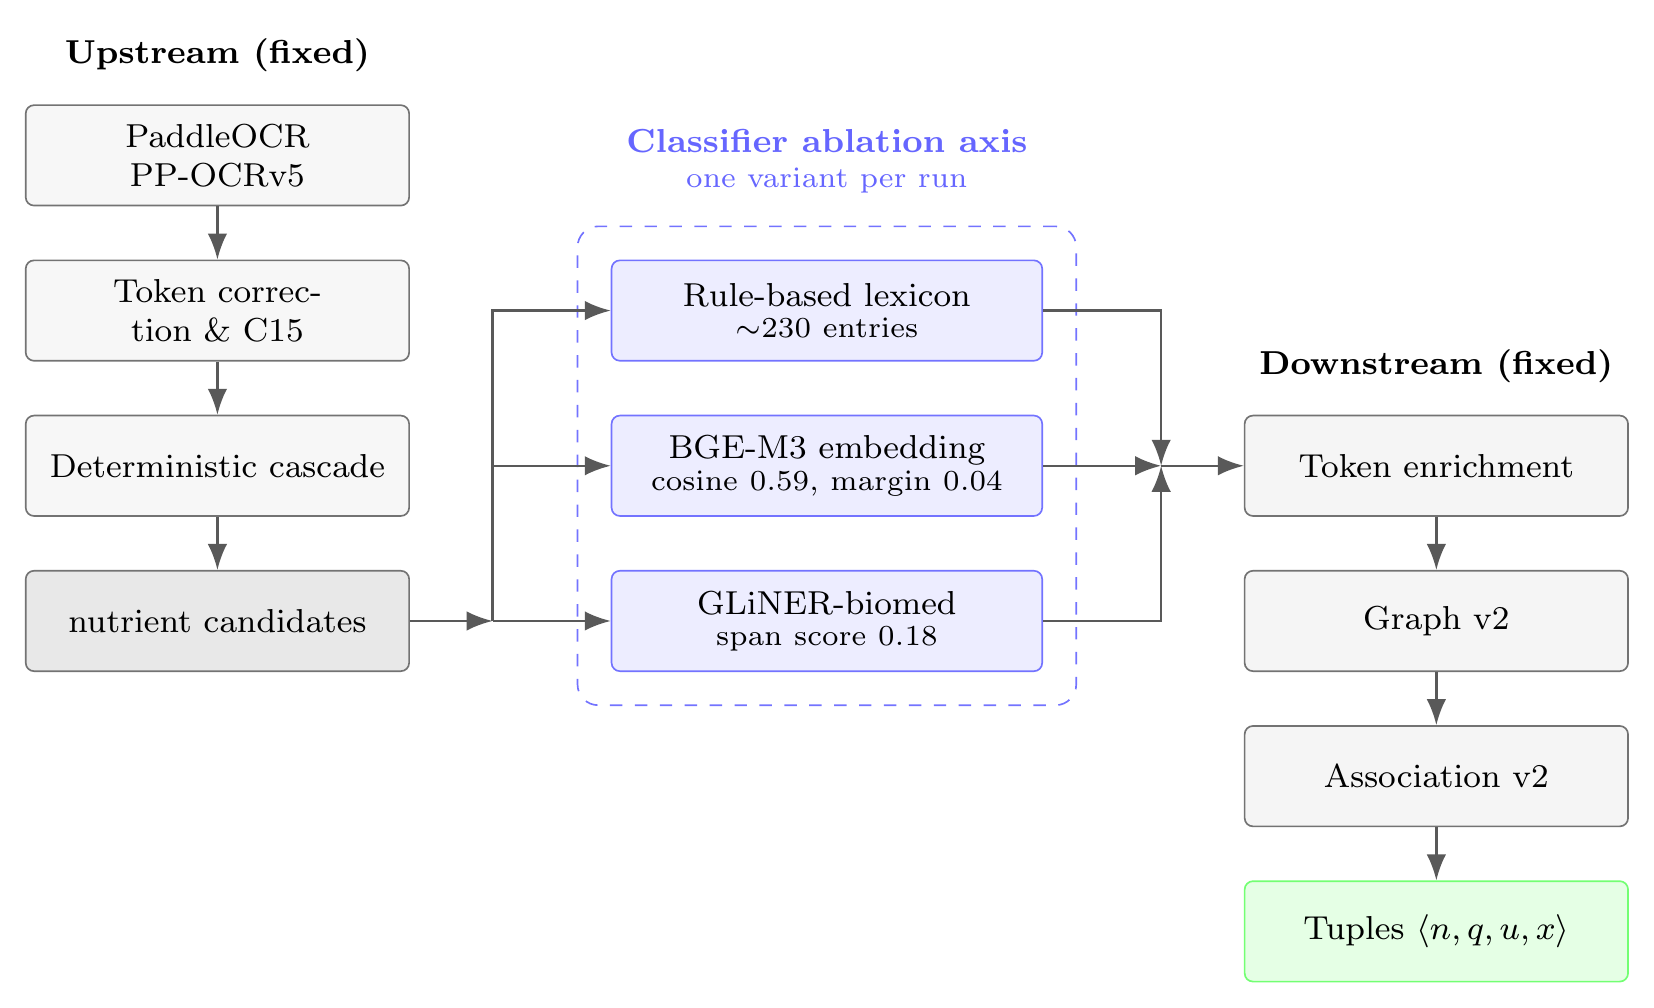
\includegraphics[width=\linewidth]{classifier_ablation.png}%
  }{%
    \fbox{\parbox[c][42mm][c]{0.92\linewidth}{\centering\itshape
      Classifier-ablation figure placeholder. Replace with
      \texttt{classifier\_ablation.png}.}}%
  }
  \caption[The semantic-classifier ablation axis]{%
    The semantic-classifier ablation axis. The upstream stages (PaddleOCR PP-OCRv5, token correction including C15, and the deterministic cascade) and the downstream stages (token enrichment, graph~v2 construction, and association~v2) are held fixed. Only the nutrient/not-nutrient decision is exchanged between the rule-based lexicon classifier, the BGE-M3 embedding classifier, and the GLiNER-biomed classifier. Exactly one classifier variant is active in any single experiment run.}
  \label{fig:classifier-ablation}
\end{figure}

\subsection{The deterministic cascade}\label{sec:classifier-cascade}

The deterministic cascade assigns roles to corrected tokens through an ordered sequence of checks. For each token, the first matching rule determines the role. This ordering is important because some tokens may satisfy more than one pattern.

The cascade first checks for short unit tokens, such as \texttt{g} or \texttt{l}. These are handled early because the correction stage may split fused values into a quantity and a short unit token. If these units were checked later, they could be mistakenly removed as noise.

The next role handled is \textsc{nrv}. This captures reference-value percentages such as \texttt{80\%} or \texttt{100\% NRV}. These values are useful for preserving label information, but they are not part of the main four-field tuple.

Context expressions are then detected and normalised. Tokens that match the context map are assigned the role \textsc{context} and mapped to canonical forms such as \texttt{per\_100g}, \texttt{per\_serving}, or \texttt{per\_daily\_dose}. Serving-size expressions are also treated as context information because they define the basis under which a quantity should be interpreted.

After the context checks, the cascade handles noise, unit-lexicon matches, and numeric quantities. Noise includes residual artefacts and isolated characters that do not provide useful information for tuple construction. Tokens that match the unit lexicon are labelled as \textsc{unit}. Numeric tokens, including integers, decimals, and comparator-prefixed values such as \texttt{<0.1}, are labelled as \textsc{quantity}.

If a token reaches the end of the cascade, it has not been recognised as a percentage, context expression, unit, quantity, or noise. At this point, it is treated as a nutrient candidate and passed to the nutrient/not-nutrient decision step. The OCR confidence remains attached to the token, but it is not used as a hard filter, since a low-confidence token may still contain useful nutritional information.

The auxiliary roles are handled differently during evaluation. The \textsc{nrv} role corresponds to the \texttt{nrv\_percent} field and is kept as additional information, but it is not part of the headline four-field score. Serving-size information is folded into \textsc{context}, because it defines the reference condition under which a nutrient quantity is reported.

\subsection{The lexicon node: rule-based classifier}\label{sec:classifier-rule}

The rule-based classifier decides whether a nutrient candidate should be assigned the role \textsc{nutrient} by checking it against a curated nutrient lexicon. The lexicon contains roughly 230 entries and covers several languages that appear in the dataset, including German, English, French, Dutch, Italian, and Spanish.

The classifier first attempts a direct lexicon match. If no exact match is found, it applies a small set of supporting heuristics. These include substring matching for longer nutrient names, tokens that begin with \texttt{vitamin}, shorthand vitamin forms such as \texttt{B12}, multilingual slash-separated forms such as \texttt{Fett / fat}, and cases where a unit has been attached to the nutrient name. For example, a token such as \texttt{energie kj} can be reduced to \texttt{energie} before the lexicon check is applied. If none of these checks succeeds, the candidate remains labelled as \textsc{unknown}.

The main advantage of this classifier is that it is fast, transparent, and easy to inspect. It also performs well when the nutrient appears in a form covered by the lexicon or one of the supporting rules. Its main limitation is coverage. Nutrient names that are missing from the lexicon, written in an unexpected form, or heavily corrupted by OCR may not be recognised. Improving this classifier therefore requires manual lexicon extension, often across several languages. This limitation motivates the comparison with the embedding-based and GLiNER-based variants.

\subsection{The embedding node: BGE-M3}\label{sec:classifier-embedding}

The embedding classifier keeps the deterministic cascade unchanged, but replaces the final lexicon-based nutrient decision with a semantic similarity test. It uses the pre-trained multilingual encoder \texttt{BAAI/bge-m3}~\cite{chen2024bgem3}. Instead of training a classifier on the target label dataset, the method represents nutrient and non-nutrient categories through short prototype phrases and compares candidate tokens to these prototypes in the embedding space.

The main positive category is \textsc{nutrient}. To avoid treating every semantically meaningful token as a nutrient, the classifier also defines non-nutrient categories as negative anchors. For each category, the candidate is compared with the corresponding prototypes, and the highest cosine similarity is used as the category score.

A candidate is not encoded only as an isolated word. Instead, it is encoded together with a small amount of row context. Tokens are grouped with nearby row neighbours using vertical-centre proximity, and the combined text is passed to the encoder. For example, a token such as \texttt{Fett} may be encoded together with nearby values as \texttt{Fett 12.5 g}. This gives the encoder more information, because a word appearing next to a quantity and unit is more likely to be part of a nutrient row.

The candidate is accepted as \textsc{nutrient} only if two conditions are met. First, its similarity to the nutrient prototypes must exceed the acceptance threshold. Second, this score must be higher than the best non-nutrient score by a defined margin. If either condition fails, the token remains \textsc{unknown}.

The embedding node can be used in two modes. In the embedding-only mode, all nutrient candidates are decided by the encoder, without using positive lexicon decisions. In the hybrid mode, the lexicon classifier keeps its positive nutrient matches, and the embedding model is used only to recover candidates that the lexicon left as \textsc{unknown}.

\subsubsection{Threshold calibration}

The embedding node uses two decision parameters: the cosine similarity threshold for accepting a token as a nutrient, and the margin over the best non-nutrient category. These parameters were selected through a token-level grid search over nutrient-candidate decisions. The calibration set contained 796 candidate decisions from the 57 label images, including 462 true nutrient tokens and 334 non-nutrient tokens.

For each threshold--margin combination, every candidate was classified either as \textsc{nutrient} or not, and the prediction was compared with the manual token-level label. Figure~\ref{fig:threshold-sweep} shows the threshold sweep for the embedding node. The best operating region was found around a cosine threshold of \(0.59\), where the token-level nutrient-classification F1 score reached approximately \(0.87\).

The margin parameter had a smaller effect than the acceptance threshold. Strong configurations generally used a small margin, usually between \(0.01\) and \(0.07\). Larger margins made the classifier more conservative, but also removed many correct nutrient names because some true nutrients still had moderate similarity to non-nutrient prototypes. Based on this sweep, the final embedding configuration uses a cosine threshold of \(0.59\) and a margin of \(0.04\).

\begin{figure}[htbp]
  \centering
  \IfFileExists{threshold_sweep.png}{%
    
\includegraphics[width=\linewidth]{threshold_sweep.png}%
  }{%
    \fbox{\parbox[c][42mm][c]{0.92\linewidth}{\centering\itshape
      BGE-M3 calibration heatmap placeholder. Replace with
      \texttt{threshold\_sweep.png}.}}%
  }
  \caption[Threshold calibration of the BGE-M3 nutrient node]{%
    Threshold--margin calibration for the BGE-M3 nutrient node. The heatmap shows token-level F1 scores across cosine similarity thresholds and margins. The black circle marks the best setting (threshold \(0.59\), margin \(0.04\); F1 = \(0.869\)), and the red cross shows the default setting (\(0.40\), \(0.10\)).}
  \label{fig:threshold-sweep}
\end{figure}


\subsection{The GLiNER node: GLiNER-biomed}\label{sec:classifier-gliner}

The third classifier variant uses GLiNER-biomed, specifically \emph{Ihor/gliner-biomed-bi-large-v1.0}~\cite{yazdani2025glinerbiomed}. Here, the model is used as a zero-shot named-entity recogniser. This means that it can receive an entity description at inference time and identify matching spans without being trained on the target supplement-label dataset.

In the proposed pipeline, the remaining nutrient candidates are passed to GLiNER using one descriptive entity label: \texttt{nutritional ingredient or vitamin or mineral}. If a candidate is covered by an accepted span for this label, it is assigned the role \textsc{nutrient}. Otherwise, it remains \textsc{unknown}. The bi-large version is used because it provided stronger zero-shot recall and more stable behaviour on German OCR text than smaller alternatives during development.

\subsubsection{Threshold calibration}

In this setup, GLiNER has one main decision parameter: the span-acceptance threshold. This threshold controls how confident the model must be before a detected span is accepted as evidence for a \textsc{nutrient} label. Unlike the BGE-M3 embedding node, the GLiNER node does not use a margin against non-nutrient categories.

The threshold was selected using the same token-level calibration approach used for the embedding classifier. Each nutrient candidate from the 57 label images was scored by GLiNER, and the predictions were compared with the manual token-level labels. Precision, recall, and token-level nutrient-classification F1 were then computed across the threshold grid. Figure~\ref{fig:threshold-sweep-gliner} shows the resulting curve for 803 candidates, consisting of 438 true nutrients and 365 non-nutrients.

The selected threshold is \(0.18\). At this operating point, the token-level nutrient-classification F1 is approximately \(0.89\), with precision \(0.91\) and recall \(0.87\). The threshold is deliberately kept relatively low because the later graph-based association stage can still reject some incorrectly connected candidates, while a nutrient missed at the classification stage cannot be recovered later.

\begin{figure}[htbp]
  \centering
  \IfFileExists{threshold_sweep_gliner_c15.png}{%
    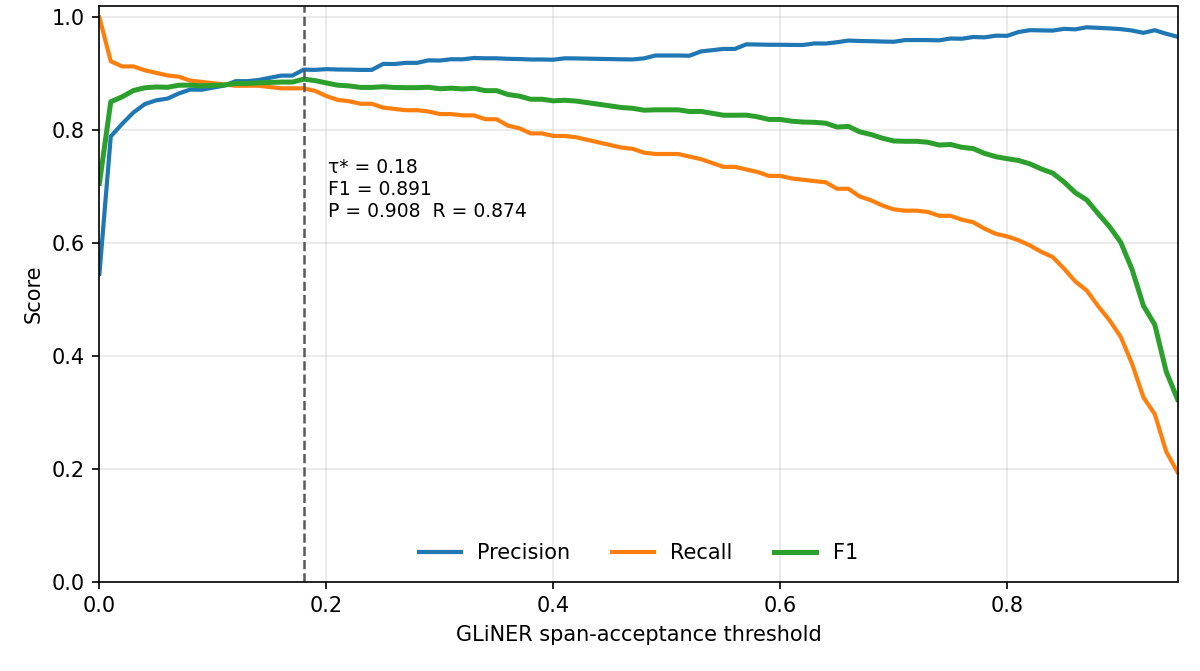
\includegraphics[width=\linewidth]{threshold_sweep_gliner_c15.png}%
  }{%
    \fbox{\parbox[c][42mm][c]{0.92\linewidth}{\centering\itshape
      GLiNER threshold-sweep placeholder. Replace with
      \texttt{threshold\_sweep\_gliner\_c15.png}.}}%
  }
  \caption[Threshold calibration of the GLiNER nutrient node]{%
    Threshold calibration for the GLiNER nutrient node. The plot shows precision, recall, and token-level nutrient-classification F1 across different span-acceptance thresholds, using 803 nutrient-candidate decisions from the 57 label images. The selected threshold is \(0.18\), which gives a token-level F1 of approximately \(0.89\), with precision \(0.91\) and recall \(0.87\).}
  \label{fig:threshold-sweep-gliner}
\end{figure}


\subsection{Choice of classifier}\label{sec:classifier-choice}

The three classifier variants were included because they represent different design choices. The rule-based classifier is the easiest to inspect and is very effective when the nutrient name is covered by the lexicon. Its limitation is that it remains a closed-vocabulary approach. A new nutrient name, spelling variant, or heavily corrupted OCR token can only be recognised if it is already covered by the lexicon or by one of the supporting rules.

The embedding classifier is less dependent on exact lexical coverage. By comparing candidate tokens with nutrient prototypes in the embedding space, it can sometimes recover nutrient names that are missing from the lexicon. However, this flexibility also introduces a risk. Tokens that are semantically related to nutrition, but are not nutrient names, may receive high similarity scores.

GLiNER provides a third alternative. It does not require a manually curated nutrient lexicon, but it can still detect nutrient-like spans from a descriptive entity label. This makes it useful for the generalisation argument of the thesis, because the classifier can be applied without training on the target label dataset and without manually adding every possible nutrient name. In the experiments, GLiNER gives performance close to the strongest classifier settings while remaining a pre-trained zero-shot component.

For this reason, the GLiNER node is treated as the main zero-shot classifier configuration in the later analysis. The embedding node is kept as a second zero-shot alternative, while the rule-based classifier is kept as a strong and transparent closed-vocabulary reference. All three classifiers are still included in the full classifier-by-association experiment matrix reported in Chapter~\ref{chap:experiments}.
% =====================================================================
%  4.4  TOKEN ENRICHMENT AND GEOMETRY
% =====================================================================

\section{Token Enrichment and Geometry}\label{sec:enrichment}

After the tokens have been classified, the pipeline knows what type of information each token may contain, but it still does not know how these pieces of information belong together on the label. A token can be marked as a nutrient, a quantity, a unit, or a context expression, but this label alone does not reveal its layout relationship to the other tokens. For example, it does not tell whether two tokens are part of the same row, whether a value belongs to a particular column, or whether a header controls the interpretation of the values beneath it. The enrichment stage is introduced to add this missing layout structure before the graph is built.

This stage extends each non-noise token with additional information that is not available from the classifier alone. Part of this information is geometric, such as the token position and its distance from nearby tokens. Another part is structural, such as the estimated row, column, column role, header status, and ordinal position within a column. These attributes are later used by the graph constructor to decide which tokens should be connected and what type of relationship each connection represents.

\subsection{Direction-aware geometry}\label{sec:enrichment-geometry}

The geometry engine does not rely only on the rectangular position of a token. Instead, it also estimates the local text direction around each token. This is particularly useful for supplement labels because the images are not always captured under ideal conditions. Labels may be slightly rotated, photographed from an angle, or printed on curved packaging, making purely axis-aligned geometric reasoning unreliable. By estimating a direction vector that follows the reading direction of each token and using this vector when comparing neighbouring tokens, the pipeline can distinguish movement along a row from movement across rows and therefore infer spatial relationships more reliably under these conditions.

For each token, the engine estimates its centre point \((c_x, c_y)\), local text angle, a direction vector along the reading direction, and a normal vector perpendicular to it. When a four-corner polygon is available, it is used for this estimation; otherwise, the token bounding box is used. This gives the pipeline a local coordinate system for comparing tokens. Movement along the direction vector roughly corresponds to movement within the same row, while movement along the normal vector corresponds more closely to movement between rows.

Two tokens are considered to belong to the same row if they point in nearly the same direction and are close to each other. The system allows small differences in angle (about \(15^\circ\)). Columns are found in a similar way, but using the other direction. This helps the system still work well even if the label is slightly rotated or photographed at an angle.

Rows and columns are then assigned using several layout modes. In the centre-coordinate (\(c_x/c_y\)) mode, a gap-based grouping strategy is used: after projecting and sorting the tokens, the algorithm starts a new row or column whenever the gap between consecutive tokens becomes too large. At the reference resolution, the row gap along the \(y\)-axis is about \(25\) pixels, while the column gap is about \(60\) pixels, and these thresholds are scaled according to the image size. Other modes are also supported, including overlap-based grouping and role-rank strategies, which use different criteria to determine row and column membership depending on the label structure.

\subsection{Structural attributes}\label{sec:enrichment-structure}

Once the approximate rows and columns have been identified, the token enricher adds a structural description to each token. This description goes beyond the token's text and position. Each token is assigned a row identifier and a column identifier, which allows the later stages to reason about the table-like structure of the label.

The columns are then interpreted using the semantic roles of the tokens they contain. For example, if most non-header tokens in a column are nutrient names, the column is treated as a nutrient-name column. If a column mainly contains numerical values, it is treated as a value column. Other columns may be interpreted as unit columns or NRV columns. This column-level information helps the graph constructor distinguish between different parts of the label instead of relying only on local token proximity.

The enrichment stage also identifies header tokens and uses them to assign context information to value columns. This is important because many nutrition and supplement labels report the same nutrients under more than one basis. For example, one column may give values per serving, while another column may give values per 100~g, per 100~ml, or per daily dose. To keep these value columns separate, the enricher can assign a dosage-stream identifier to each context-bearing value column. In this way, the graph stage can treat different value columns as separate streams rather than mixing quantities that belong to different contexts.

Several rank-based attributes are also computed. Each token receives a rank within its row, a rank within its column, and a role-specific rank. The column rank is calculated over non-header tokens, while the role-specific rank is calculated separately for roles such as \textsc{nutrient}, \textsc{quantity}, and \textsc{unit}. These ranks are not the main mechanism for association, but they provide useful fallback information and allow alternative edge-construction modes to be tested in the graph stage.

The enriched tokens also keep confidence values for row and column membership. This is useful because the layout is not always clear. Some labels have irregular spacing, weak table boundaries, or mixed paragraph-and-table formatting, so assigning a token to a row or column may be uncertain.

The enricher assumes that the main nutritional information in an image is mostly contained in one table-like region. This assumption fits most labels in the dataset, but it is still a simplification. When a label contains multiple separate tables, or when table entries are mixed with paragraph text, some structural attributes may become less reliable. For this reason, the graph stage does not depend only on the induced table structure. It also keeps geometric relations and fallback routes, which makes the association process more robust when the structural enrichment is imperfect.

\subsection{Two views of the row relation}\label{sec:enrichment-rowviews}

The row relation is one of the most important layout cues for tuple reconstruction. In many nutrition and supplement tables, a nutrient is associated with a quantity simply because both appear on the same printed row. The enrichment stage therefore provides two ways to describe this relation before the graph is built.

The first view is geometric. Two tokens are considered related when they are aligned in the image. On clean labels, this can be approximated by comparing their \(c_y\) positions. A more robust criterion is to consider the extent they share along the vertical axis: tokens whose vertical spans have a large common extent are likely to belong to the same row, even when their heights differ. This criterion remains effective even when the label contains moderate distortions or variations in token size. In all cases, the row relation is derived directly from the visual layout of the label.

The second view is structural. Instead of relying only on pixel alignment, this view uses the ordinal order of tokens inside their columns. For example, the first nutrient can be paired with the first quantity, the second nutrient with the second quantity, and so on. This can work well when the columns are correctly detected and when the entries in each column follow the same order. In such cases, ordinal rank provides another way to recover the row relation, even if the visual alignment is not perfectly clean.

In practice, the structural view is more fragile than it may first appear. OCR errors can easily disturb the one-to-one ordering between nutrient, quantity, and unit columns. If a token is missed, one column becomes shorter than the others. If a quantity and unit are fused into one token, the expected unit sequence may change. Extra tokens, such as NRV percentages, footnote markers, or OCR artefacts, can also shift the rank count. The same problem can occur when the column detection itself is imperfect and the rank is computed over the wrong group of tokens.

Once the ordering is shifted, the error can propagate through the rest of the table. For example, if one quantity is missing near the top of a value column, the nutrients below it may be matched with quantities from neighbouring rows. This is particularly harmful for the quantity field, because quantities usually differ from row to row. Unit values, on the other hand, may still appear correct even when the row association is wrong, since many nutrients share repeated units such as \texttt{mg}. For this reason, a high unit score under rank-based pairing does not necessarily prove that the row matching itself is correct.

The geometric view is less sensitive to this type of OCR error. If one token is missing, fused, or falsely added, the remaining tokens still stay close to their printed row. A quantity that is visually aligned with a nutrient remains aligned, even if another entry above it is missing. Therefore, the graph uses geometric row edges as the main representation of the row relation, while ordinal ranks are kept only as fallback or experimental information. The edge-construction modes based on these two views are described in Section~\ref{sec:graph}, and their effect is evaluated in Chapter~\ref{chap:experiments}.

% =====================================================================
%  4.5  SEMANTIC GRAPH CONSTRUCTION
% =====================================================================
\section{Semantic Graph Construction}\label{sec:graph}

After the enrichment stage, each token carries more than just text. It now has a semantic role, geometric information, and structural attributes such as row or column membership. The next step is to represent these enriched tokens as a graph. The purpose of this graph is to make the possible relationships between tokens explicit before the final association step. Instead of searching over an unstructured list of OCR tokens, the matcher receives a graph that already indicates which tokens are likely to be aligned in the same row, belong to the same column, appear near each other, or fall under the same contextual scope.

In this graph, the nodes correspond to the non-noise tokens. The edges represent typed relationships between these tokens. These edges do not directly define the final output tuples, but they narrow and organise the search space for the association stage. For example, a row edge between a nutrient and a quantity suggests a possible nutrient--quantity relation. An adjacency or row edge between a quantity and a unit suggests a possible quantity--unit relation. Similarly, an edge from a context header to a value-bearing token can indicate the reference basis under which the value should be interpreted.

Two graph constructors are evaluated in this thesis. The first constructor, referred to as graph~v1, is the simpler variant. It builds relations using the classified tokens and their raw bounding-box geometry. The second constructor, graph~v2, uses the enriched representation described in Section~\ref{sec:enrichment}. This allows graph~v2 to use additional information such as row and column identifiers, column roles, ordinal ranks, dosage-stream identifiers, header flags, and direction-aware geometry. Figure~\ref{fig:graph-constructors} illustrates the difference between the two graph construction variants.

\begin{figure}[htbp]
  \centering
  \IfFileExists{graph_constructors.png}{%
    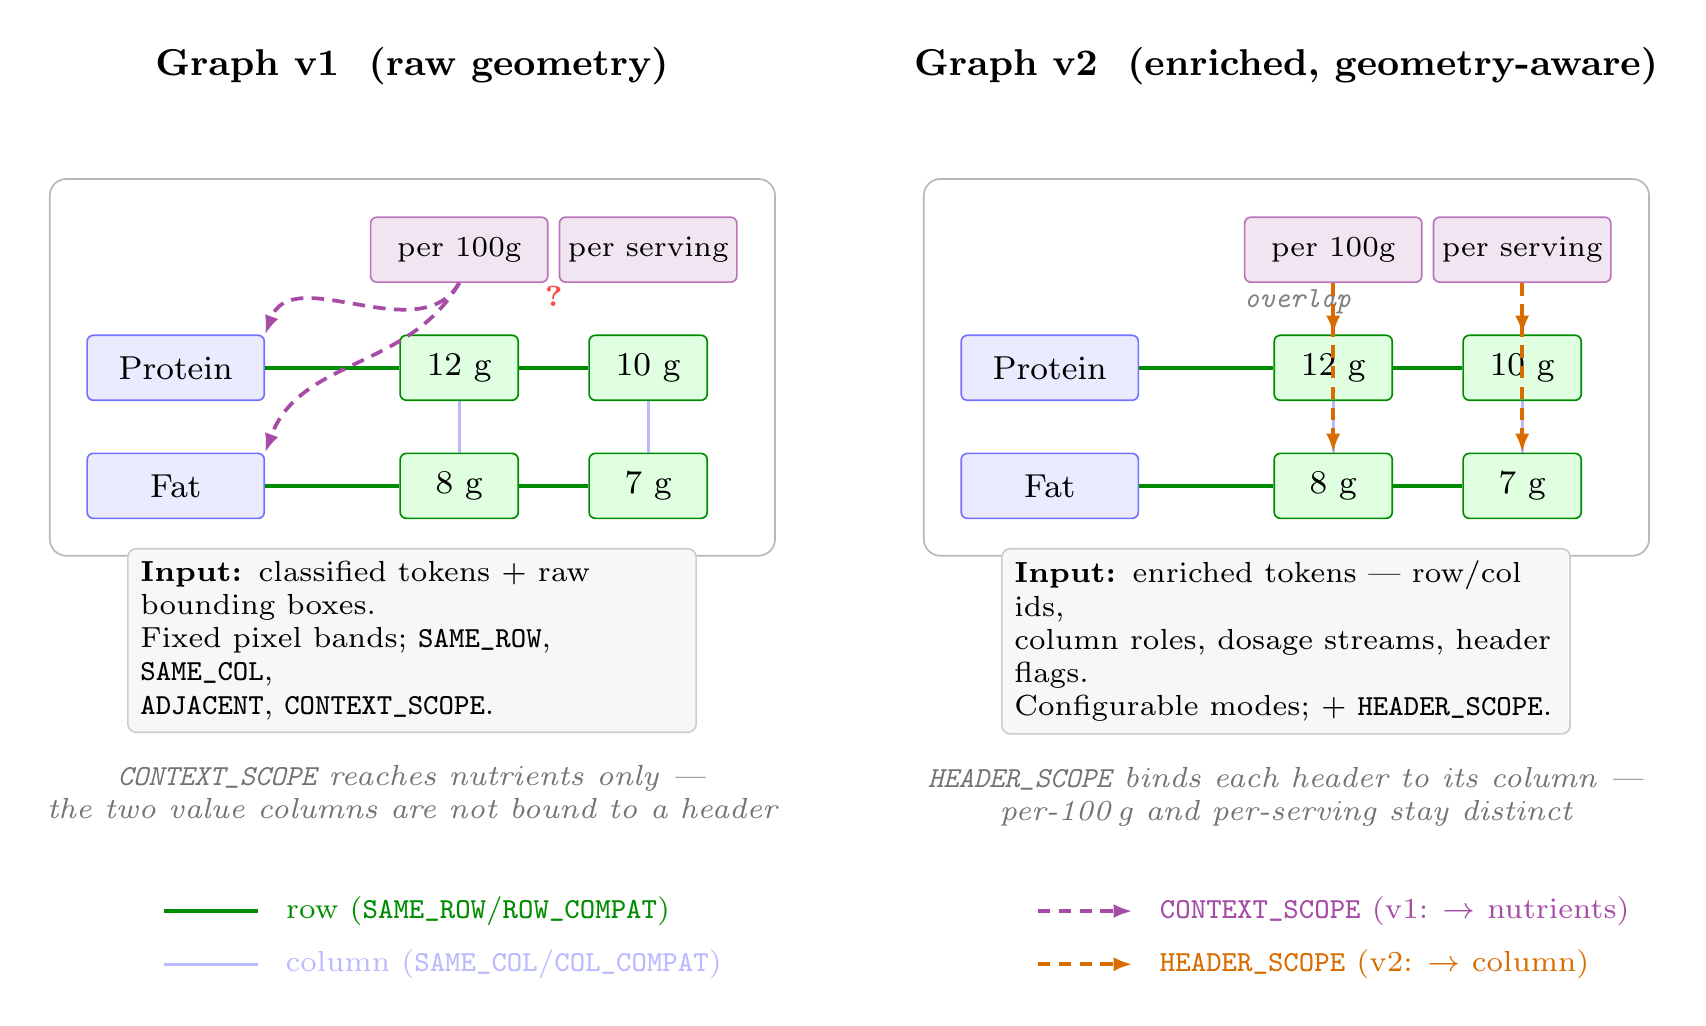
\includegraphics[width=\linewidth]{graph_constructors.png}%
  }{%
    \fbox{\parbox[c][52mm][c]{0.92\linewidth}{\centering\itshape
      Graph-constructor comparison figure placeholder. Replace with
      \mcode{graph_constructors.png}.}}%
  }
  \caption[Graph v1 and graph v2]{%
    Comparison of the two graph constructors on a label with two value columns. Graph~v1 builds edges from raw bounding-box geometry, and its context-scope edge edge reaches nutrient nodes only, so the two value columns are not bound to their respective headers. Graph~v2 uses the enriched token structure; its header-scope edge edge binds each header to the tokens in its own column, keeping the per-100\,g and per-serving contexts distinct.}
  \label{fig:graph-constructors}
\end{figure}

\subsection{Graph v1: the naive constructor}\label{sec:graph-v1}

Graph~v1 is used as the simple geometry-based baseline. It operates directly on the classified OCR tokens, without using the enriched representation described in Section~\ref{sec:enrichment}. Each non-noise token is converted into a graph node, and its centre point \((c_x, c_y)\) is recomputed from the token bounding box. The constructor therefore ignores the induced row and column identifiers, column roles, ordinal ranks, dosage streams, and header flags produced by the enrichment stage.

The edge set in graph~v1 is deliberately limited. It contains four main types of relations. The first is  same-row edge. This edge is added when two tokens have similar vertical centre positions, using a row band of approximately \(25\) pixels. The second relation is  same-column edge, which connects tokens whose horizontal centres are close to each other, using a narrower band of approximately \(20\) pixels.

The third relation is  adjacency edge. This edge is added when two token boxes are spatially close, with a distance threshold of approximately \(60\) pixels, and when no row or column edge has already been created between them. In practice, this relation acts as a fallback. For example, a unit may be slightly shifted away from its quantity because of OCR segmentation. Even if it does not satisfy the row or column criteria, it may still be recovered through an adjacency edge.

The fourth relation is context-scope edge. This is a directed edge from a context token to nutrient tokens below it, within a vertical range of approximately \(600\) pixels. The purpose of this edge is to allow a header or context phrase to influence the nutrient entries that appear underneath it.

All thresholds in graph~v1 are based on pixel distances, scaled according to the image height. This makes the constructor easy to understand and useful as a baseline, but it also limits its ability to represent the real structure of dense supplement labels. It treats the page mainly as a set of coordinates and does not use the table structure inferred during enrichment. As a result, graph~v1 cannot distinguish between different sources of row or column evidence. Its role in the experiments is therefore to show what can be achieved with simple geometric relations before adding the enriched structural information used in graph~v2.

\subsection{Graph v2: the geometry-aware constructor}\label{sec:graph-v2}

Graph~v2 uses the enriched token representation produced in the previous stage. Each node keeps the token text, semantic role, geometry, row and column identifiers, column role, ordinal ranks, dosage-stream identifier, and header flag. Unlike graph~v1, this constructor does not rely only on recomputing relations from the bounding boxes. Instead, it uses the layout and structural information already added during enrichment.

Because of this richer input, graph~v2 also defines a richer set of edge types. The main relations are  row-compatibility edge,  column-compatibility edge , directional-adjacency edge, context-scope edge, and header-scope edge. The main difference from graph~v1 is that row and column compatibility are no longer based on one fixed pixel-band rule. They can be created through different edge-construction modes, which makes it possible to compare geometric and structural interpretations of the label layout.

The row relation,  row-compatibility edge, can be built in several ways. The default mode is \mcode{overlap}. This is a geometric mode based on the shared vertical extent of two token boxes. Two tokens receive a row edge when the intersection of their vertical spans \([y_1, y_2]\) covers at least \(0.30\) of the shorter span. This threshold was selected by a coordinate-descent sweep over the three overlap thresholds, shown in Figure~\ref{fig:overlap-sweep}, in which the row threshold is the decisive axis while the column and context thresholds are nearly flat. The overlap criterion is more stable than comparing only the vertical centre points, because two tokens can still belong to the same printed line even when their bounding-box heights differ. A second geometric mode, vertical-centre mode, links tokens when the distance between their vertical centres is within a fixed band of approximately \(25\) pixels, although the effective tolerance depends on the resolution of the input image. Both geometric modes work as pairwise checks. Figure~\ref{fig:row-modes} contrasts the four row modes on a label where one quantity has been dropped by OCR.

The  role-rank mode mode is a structural mode that counts the order separately for each semantic role. In this mode, the \(k\)-th nutrient, the \(k\)-th quantity, and the \(k\)-th unit can be linked together. Since same-column links are allowed, this mode can recover some inline quantity--unit relations. However, it still depends on the ordinal sequence being correct, so it can fail when OCR errors shift the role-specific ranks.

The \mcode{role_rank_cy} mode combines the structural and geometric views. It creates a row edge when the role-specific ranks match, or when the tokens are geometrically aligned on the same row. This mode was included because pure rank matching and pure geometry handle different failure cases. The rank component can preserve some inline unit links, while the geometric component can recover visually aligned tokens even when the rank sequence has been disturbed.

\begin{figure}[htbp]
  \centering
  \IfFileExists{row_modes.png}{%
    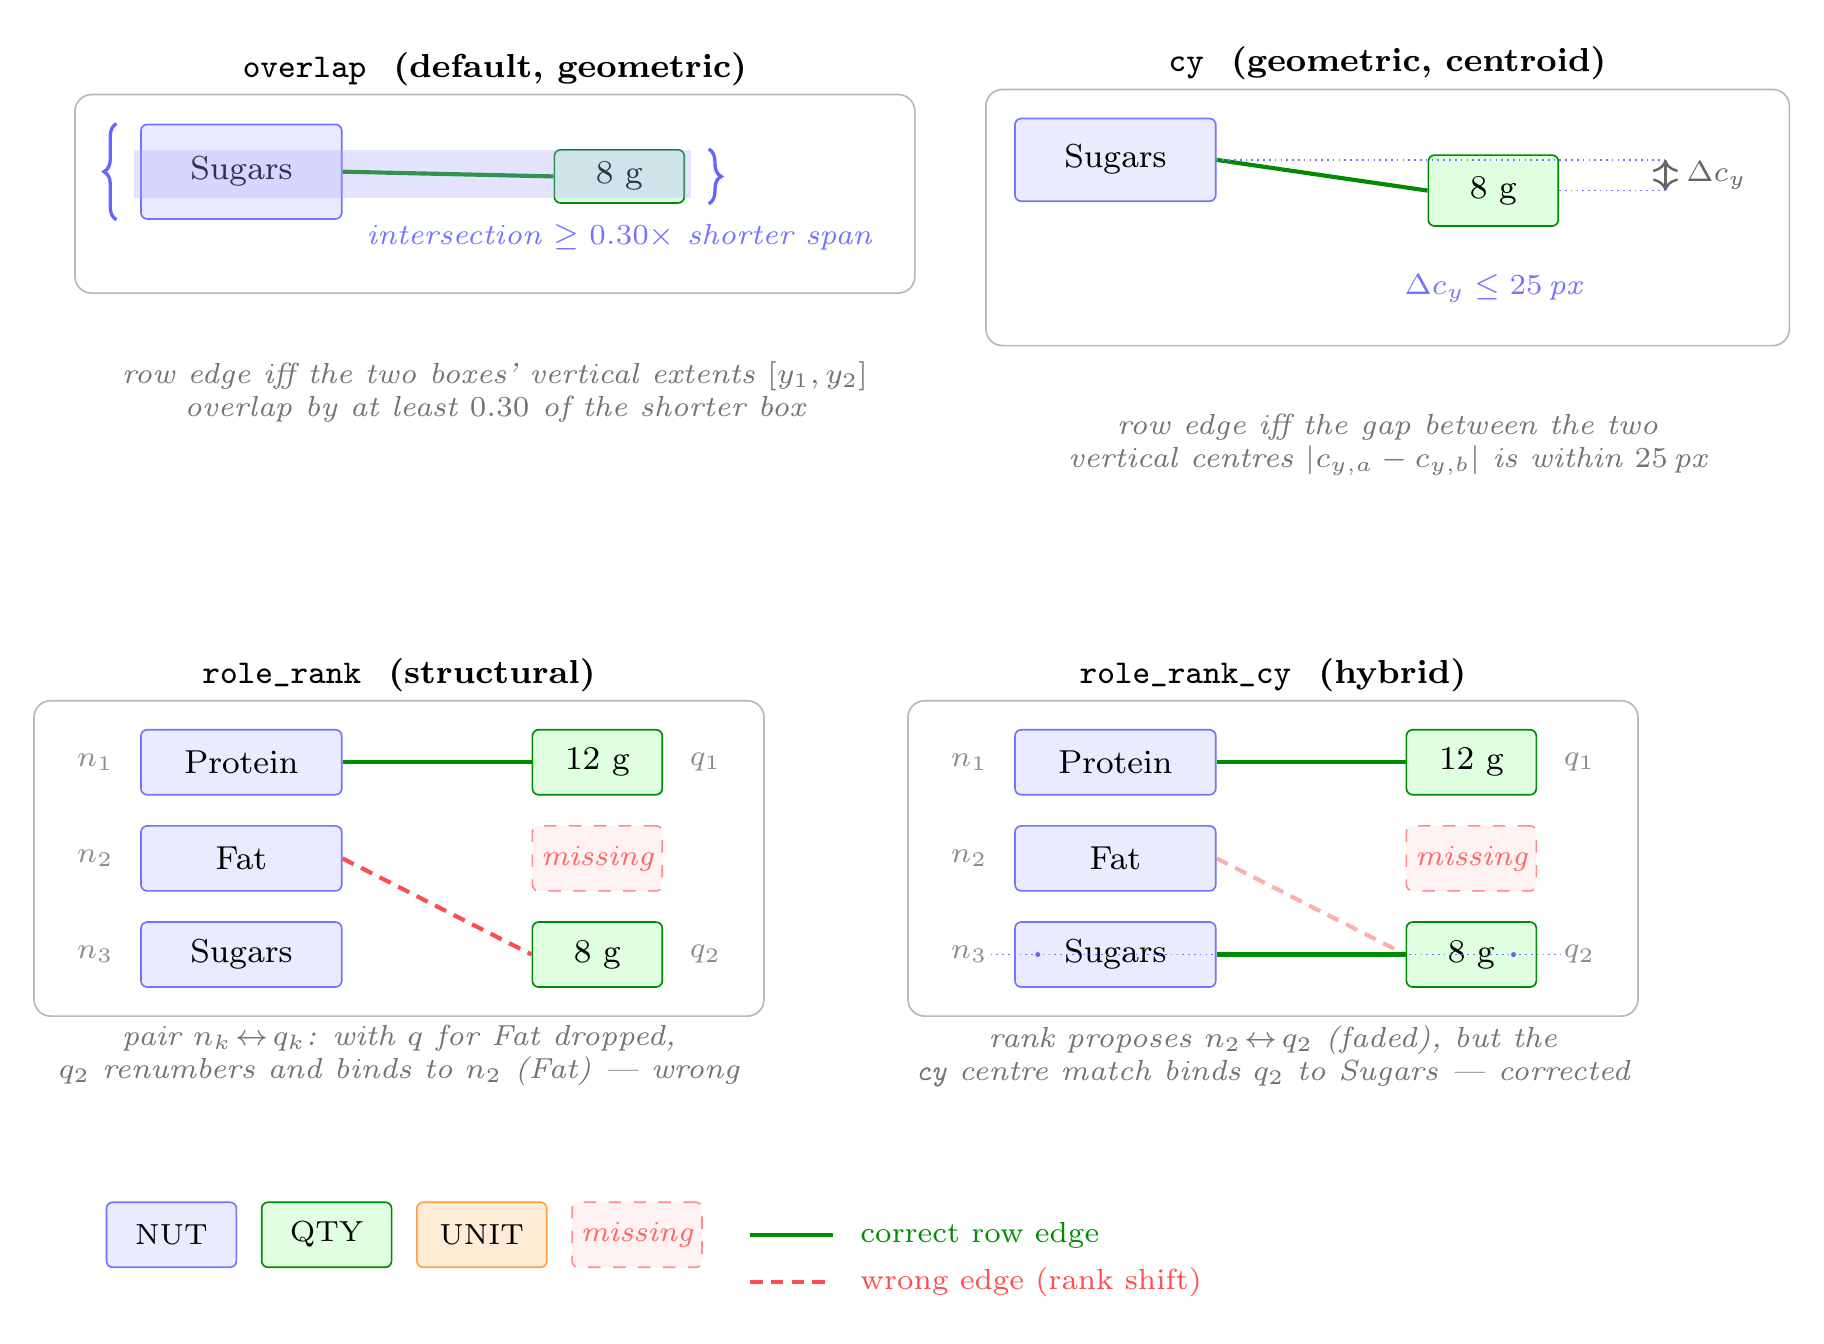
\includegraphics[width=\linewidth]{row_modes.png}%
  }{%
    \fbox{\parbox[c][55mm][c]{0.92\linewidth}{\centering\itshape
      Row-mode comparison figure placeholder. Replace with
      \mcode{row_modes.png}.}}%
  }
  \caption[The four  row-compatibility edge modes]{%
    The four  row-compatibility edge edge-construction modes on the same input, where the quantity of \emph{Fat} has been dropped by OCR. The geometric modes \mcode{overlap} and vertical-centre mode link each quantity to its visually aligned nutrient and correctly leave \emph{Fat} unmatched; \mcode{overlap} decides on the intersection of the two boxes' vertical extents, while vertical-centre mode decides on the gap between their vertical centres. The structural mode  role-rank mode pairs the \(k\)-th nutrient with the \(k\)-th quantity, so the missing entry renumbers \(q_2\) and binds the \mcode{8\,g} value to \emph{Fat}. The hybrid mode  role-rank plus vertical-centre mode would propose the same incorrect rank link, but the geometric alignment overrides it and restores the correct row.}
  \label{fig:row-modes}
\end{figure}

The column relation,  column-compatibility edge, is constructed using a smaller set of modes. The default mode is \mcode{overlap}, which connects tokens when the intersection of their horizontal spans \([x_1, x_2]\) covers at least \(0.20\) of the shorter span. The horizontal-centre mode mode is a centre-based alternative that links tokens whose horizontal centres are within a fixed band of approximately \(20\) pixels. A third option,  column-identifier mode, uses the column identifiers assigned during enrichment. These modes allow the experiments to test whether shared horizontal extent, centre proximity, or induced column structure is more useful for the association task.

Context handling is also improved in graph~v2. The context-scope edge edge links a context token to relevant tokens in its scope, but it is no longer limited to nutrient nodes. It can also reach quantities and units, which is important because the context usually defines the basis of a value, not only the nutrient name. This edge also uses a lateral gate. In the default \mcode{overlap} setting, the context token and the governed token must share at least \(0.10\) of their horizontal extent. In the vertical-centre mode setting, no lateral gate is applied, and the edge is based only on vertical scope.

Graph~v2 also introduces the header-scope edge edge. This relation uses the induced column structure to connect detected headers with the tokens in the same column. It is especially useful when a label contains multiple value columns with different contexts. For example, one column may report values per 100~g, while another reports values per serving. If both headers appear at a similar vertical position, a purely vertical context rule may not separate them reliably. The column-based header relation gives the graph another way to keep these context streams distinct.

\begin{figure}[htbp]
  \centering
  \IfFileExists{calib_overlap_sweep.png}{%
    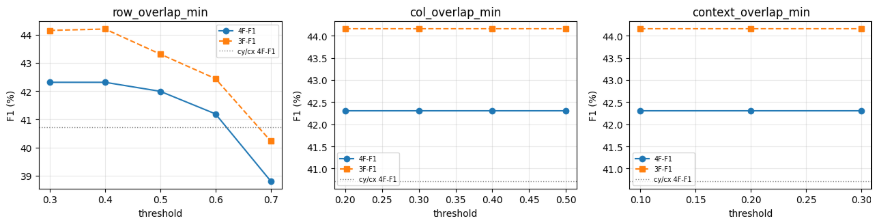
\includegraphics[width=\linewidth]{calib_overlap_sweep.png}%
  }{%
    \fbox{\parbox[c][40mm][c]{0.92\linewidth}{\centering\itshape
      Overlap-threshold sweep placeholder. Replace with
      \mcode{calib_overlap_sweep.png}.}}%
  }
  \caption[Overlap-threshold calibration for graph~v2]{%
    Coordinate-descent calibration of the three \mcode{overlap} thresholds in graph~v2, sweeping one threshold at a time while holding the other two fixed. Each panel reports 4F-F1 and 3F-F1 against the swept value; the dotted line marks the vertical-centre mode/horizontal-centre mode centroid baseline. The row threshold is the decisive axis: 4F-F1 peaks at minimum row overlap ~$=0.30$ and degrades beyond it, whereas minimum column overlap  and minimum context overlap  are flat, confirming the values \(0.20\) and \(0.10\). These operating points define the default \mcode{overlap} configuration.}
  \label{fig:overlap-sweep}
\end{figure}

\subsection{What graph v2 adds}\label{sec:graph-summary}

Overall, graph~v2 extends graph~v1 by using the enriched token representation rather than only raw bounding-box geometry. This allows the graph to use configurable row and column relations, structural attributes such as column roles and dosage streams, and more direct context links through context-scope edge and header-scope edge. In the experiments, graph~v1 is therefore kept as the simple geometry-based baseline, while graph~v2 is used to test whether the additional enrichment and context-aware edge construction improve tuple association.
% =====================================================================
% 4.6 GRAPH MATCHING AND ASSOCIATION
% =====================================================================
\section{Graph Matching and Association}\label{sec:association}

The final graph-based stage converts the semantic graph into the output tuples. At this stage, the pipeline has already identified the token roles and created typed edges between related tokens. What remains is the actual association problem: selecting the quantity that belongs to each nutrient, attaching the correct unit to that quantity, and assigning the context under which the value should be interpreted.

The association stage is deterministic and zero-shot. It does not learn parameters from the target dataset, and it does not optimise a global objective over the full table. Instead, it follows a local greedy strategy. Each nutrient node is processed in turn, and the associator searches its graph neighbourhood for plausible quantities, units, and context tokens. This design keeps the behaviour simple to inspect during error analysis, although it also means that some conflicts between competing associations are not resolved globally.

Two graph-based associators are used. The first is paired with graph~v1, the naive geometry-based constructor. The second is paired with graph~v2, the enriched geometry-aware constructor. Both associators follow the same general traversal logic, but the graph~v2 associator can use richer edge types and token attributes to handle more complex layouts.

\subsection{The shared traversal core}\label{sec:association-core}

Both graph-based associators start from a nutrient node. For each token labelled as \textsc{nutrient}, the associator searches the graph for related \textsc{quantity} nodes, mainly through row-compatible edges. Candidate quantities are ordered from left to right, which is useful in multi-column labels where values often appear in a meaningful column order.

If no suitable quantity is found through the row relation, the associator uses fallback paths through column-related and nearby edges. This helps in cases where the quantity is visually separated from the nutrient, or where a row edge was missed because of OCR segmentation or irregular spacing.

After a quantity is selected, the associator resolves the remaining fields. The unit is selected using a short fallback chain that checks fused units, same-row units, nearby units, and finally units on the nutrient row. The context is resolved after the quantity and unit, with priority given to context information close to the value side. This is important because, in multi-column tables, the context is often attached to the value column rather than to the nutrient name itself.

For each resolved association, the system emits a tuple \((n, q, u, x)\). Duplicate outputs are removed when multiple graph paths lead to the same nutrient--quantity association. However, the associator does not enforce a global one-to-one matching across the whole table. It remains a greedy local method, which keeps the process simple and inspectable but may leave some conflicts unresolved.

\subsection{Extensions in the graph v2 associator}\label{sec:association-v2}

The graph~v2 associator keeps the same general traversal idea, but adds several mechanisms for more complex layouts. The first addition is per-quantity context. Since graph~v2 allows context-scope edge and header-scope edge edges to reach value-bearing tokens, different quantities on the same nutrient row can receive different contexts. This is useful when one column reports values per 100~g, while another reports values per serving or per daily dose.

The second addition is dosage-stream matching. When the enrichment stage separates value columns into different dosage streams, graph~v2 can associate the same nutrient with values from each stream separately. This allows the system to output multiple tuples for the same nutrient when the label reports it under different contexts.

The third addition is unit refinement. Instead of taking the first suitable unit found by the fallback chain, graph~v2 prefers the unit closest to the right of the quantity on the same tight line. This reduces errors in dense tables where a loose row relation may include a unit from a neighbouring row.

The fourth addition is energy-aware filtering. Energy rows are treated as a special case because they are usually reported in \mcode{kJ} or \mcode{kcal}. When the nutrient is an energy term, such as \mcode{Energie}, \mcode{Brennwert}, or \mcode{energy}, the associator prefers quantities with energy units and avoids capturing nearby gram or milligram values.

These additions make graph~v2 better suited for multi-column and context-rich supplement labels. Graph~v1 remains useful as a simpler baseline, while graph~v2 tests the value of the enriched graph representation during association.

\subsection{Fallback extraction for non-tabular layouts}\label{sec:association-fallback}

A regex-based fallback is included for cases where OCR returns paragraph-like text rather than separated table cells. It is activated only when the graph stage produces very few tuples compared with the number of detected quantities. The fallback scans the fused text for multilingual nutrient names followed by quantity--unit groups and emits the corresponding tuples directly.

This fallback improves recall on labels where the table structure is not available in the OCR output. However, it remains limited by OCR quality and does not replace the graph-based association used for table-like layouts. Remaining errors from these cases are discussed later in Chapter~\ref{chap:experiments}.
% =====================================================================
% 4.7 VISION--LANGUAGE ASSOCIATION FROM AN INJECTED TOKEN TABLE
% =====================================================================
\section{Vision--Language Association from an Injected Token Table}\label{sec:vlm-assoc}

The third association variant replaces the graph traversal step with a vision--language model. The earlier parts of the pipeline are kept unchanged: the label image is still processed by OCR, the detected tokens are corrected, and semantic roles are assigned. The difference appears only at the final association stage. Instead of using graph edges to form tuples, the corrected token table is passed to the model, and the model is asked to decide how the tokens should be grouped into nutrient tuples.

This variant is included mainly as a point of comparison rather than as the primary approach of the thesis. The idea is to see whether a general-purpose vision--language model can carry out the binding step when it is given exactly the same OCR-derived information as the graph matcher. One important limitation, however, is that the model behaves largely as a black box. It can produce the final nutrient tuples, but it does not explain why a specific nutrient was paired with a particular quantity. In contrast, the graph-based approaches provide a much clearer and more interpretable association process, since the connections can be traced through explicit graph paths and edges.

\subsection{The injected prompt}\label{sec:vlm-assoc-prompt}

The model receives the original label image together with an injected token table. Each row in the table represents one surviving token and contains its index, text, semantic role, and pixel coordinates. Tokens labelled as \textsc{nrv} or \textsc{noise} are removed before injection, so the table focuses only on the four roles needed for tuple construction: nutrient, quantity, unit, and context. The structural attributes produced by the enrichment stage are not included by default.

The prompt treats the problem as one of association rather than text recognition. The model is explicitly told to rely on the injected token table for the textual content and to use the image only for visual cues such as alignment, proximity, and table headers. This setup was chosen to keep the comparison with the graph-based approaches fair, since those methods also work solely with the OCR tokens produced in earlier stages. For this variant, Gemma 3 4B~\cite{gemma3} is used through a locally hosted OpenAI-compatible endpoint. The generation temperature is kept low to encourage more consistent outputs.

\subsection{Output and normalisation}\label{sec:vlm-assoc-output}

The model is instructed to return a bare JSON array. Each object in the array contains four fields: \texttt{nutrient}, \texttt{quantity}, \texttt{unit}, and \texttt{context}. The prompt also requires the model to use only information from the injected token table and to avoid creating associations that are not supported by the provided tokens. If the response is cut off because of the token limit, the parser attempts to recover any complete JSON objects from the partial output.

Before evaluation, the predicted tuples are normalised. Quantity and unit strings are lightly cleaned, and context values are mapped to canonical forms such as \mcode{per_100g} and \mcode{per_serving}. Nutrient names are normalised using the same C15 mapping used elsewhere in the pipeline.

The placement of C15 is important in this variant. In the graph-based paths, C15 is applied before association, so the matcher works directly with canonical nutrient names. In the vision--language path, the token table is injected before C15 is applied. This choice is intentional. The model also sees the original image, where the text still appears in its original surface form, for example \texttt{Eiwei{\ss}} or \texttt{davon Zucker}. If the injected table had already replaced these forms with \texttt{Protein} or \texttt{Sugars}, the token text would no longer match what is visible in the image. For this reason, the VLM first receives the corrected surface forms, and C15 is applied only after the model has produced its tuples. This keeps the VLM input consistent with the image while still evaluating all variants using the same canonical vocabulary.